\begin{center}
	\begin{circuitfig}[H]
		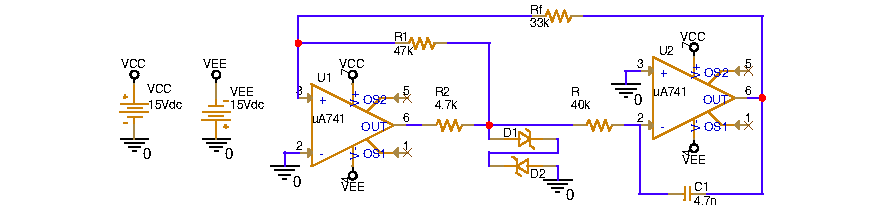
\includegraphics[width=15cm]{spice_01/schematic.pdf}
		\caption{Κύκλωμα προσομοίωσης για το PSpice.}
		\label{circ:spice:1_schematic}
	\end{circuitfig}
\end{center}
\vspace*{-10pt}

Οι προσομοιώσεις έγιναν με το κύκλωμα \ref{circ:spice:1_schematic}. Οι δίοδοι Zener\footnote{Χρησιμοποιήθηκαν δεδομένα από data sheet της διόδου 1N5236B του εμπορίου.}, D1 και D2, δημιουργήθηκαν χρήσει του \textsl{PSpice Modeling Application}. Η τάση Zener των διόδων ορίστηκε $V_Z=7.5\unit{\volt}$ και ο θερμοκρασιακός συντελεστής ορίσθηκε στο $0.058\displaystyle{\sfrac{\%}{\unit{\celsius}}}$.

\begin{chart}[H]
	\begin{center}
		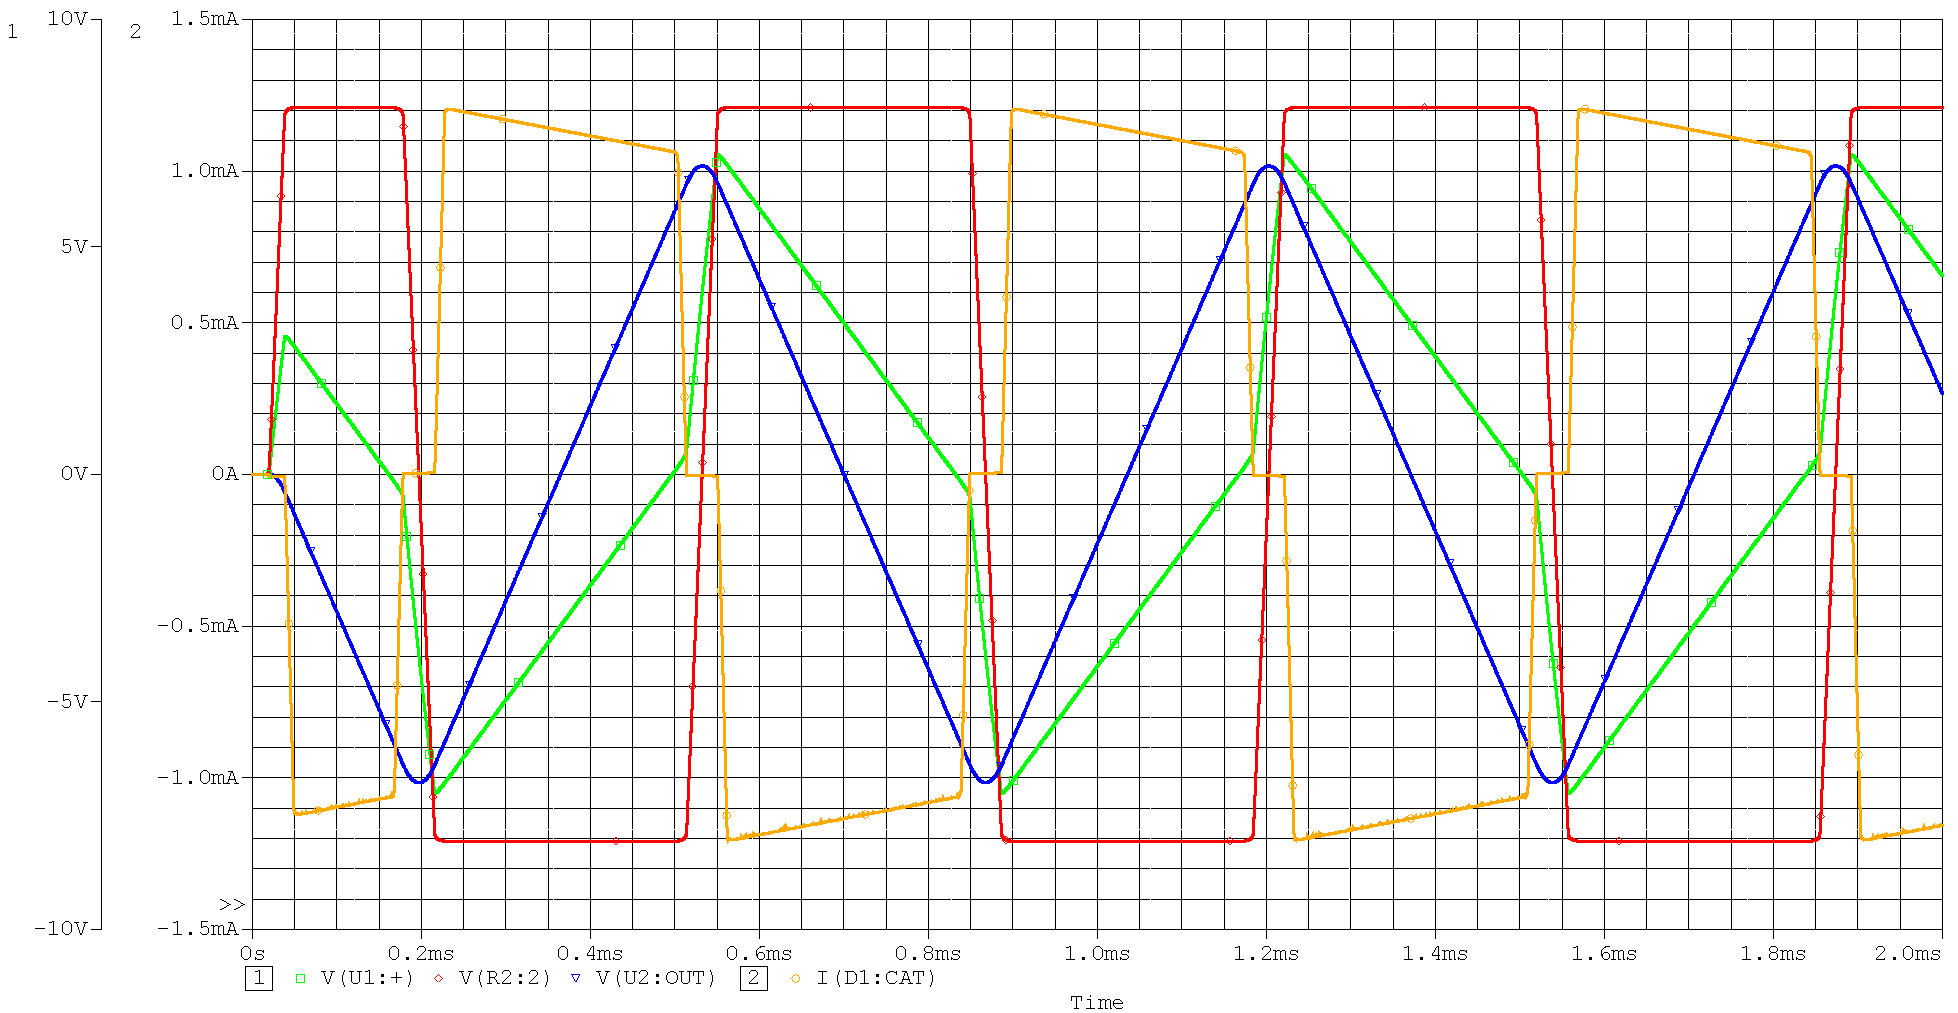
\includegraphics[width=15cm]{spice_01/q4cropped.pdf}
		\caption{Οι τάσεις $V_1$ (πράσινη κυματομορφή), $V_2$ (κόκκινη κυματομορφή) και $V_{\mathrm{out}}$ (μπλε κυμματομορή) και το ρεύμα $I_Z$ (πορτοκαλί κυματομορφή).}
		\label{plot:ask1:q4}
	\end{center}
\end{chart}

Οι περίοδοι των κυματομορφών βρέθηκαν με τη βοήθεια των cursors ενώ τα μέγιστα και ελάχιστα των κυματομορφών βρέθηκαν χρήσει των συναρτήσεων \texttt{Max()} και \texttt{Min()}. Τα αποτελεσματα φαίνονται στον πίνακα \ref{table:ask1:q4:periods}.

\begin{table}[h]
	\begin{center}
		\begin{tabular}{|c|c|c|c|c|}
			\hline
			\textbf{Σήμα}      & \textbf{Περίοδος}             & \textbf{Μέγιστη τιμή}         & \textbf{Ελάχιστη τιμή}         & \textbf{Ελάχιστη τιμή}                       \\
			\hline
			\hline
			$V_1$              & $670.669\unit{\micro\second}$ & $7.02052\unit{\volt}$         & $-7.01512\unit{\volt}$         & $14.03564\unit{\volt}_{\mathrm{pp}}$         \\\hline
			$V_2$              & $670.707\unit{\micro\second}$ & $8.06550\unit{\volt}$         & $-8.06549\unit{\volt}$         & $16.13099\unit{\volt}_{\mathrm{pp}}$         \\\hline
			$V_{\mathrm{out}}$ & $670.707\unit{\micro\second}$ & $6.77889\unit{\volt}$         & $-6.77670\unit{\volt}$         & $13.55559\unit{\volt}_{\mathrm{pp}}$         \\\hline
			$I_Z$              & $670.709\unit{\micro\second}$ & $1.20446\unit{\milli\ampere}$ & $-1.20582\unit{\milli\ampere}$ & $2.41028\unit{\milli\ampere}_{\mathrm{pp}}$ \\\hline
		\end{tabular}
		\caption{Μετρήσεις των κυματομορφών του διαγράμματος \ref{plot:ask1:q4}.}
		\label{table:ask1:q4:periods}
	\end{center}
\end{table}